\chapter{Einleitung}

% \section{Motivation}

Die autonome mobile Robotik ist heutzutage nicht mehr wegzudenken und hat eine wichtige Rolle eingenommen. Die mobilen Roboter nehmen banale Aufgaben wie Staubsaugen bzw. Wischen (siehe \autoref{fig:mobileRoboterPrivaterHaushalte}), aber auch komplexere Aufgaben in der Logistik und Industrie (siehe \autoref{fig:mobileRoboterIndustrie}) wahr. Der Einsatz der Roboter soll auch in den kommenden Jahren eine wichtige Rolle bei Katastrophen wie Brand übernehmen. \cite{Retungsroboter.2019} 

\begin{figure}[H]%
  \centering
  \subfloat[][]{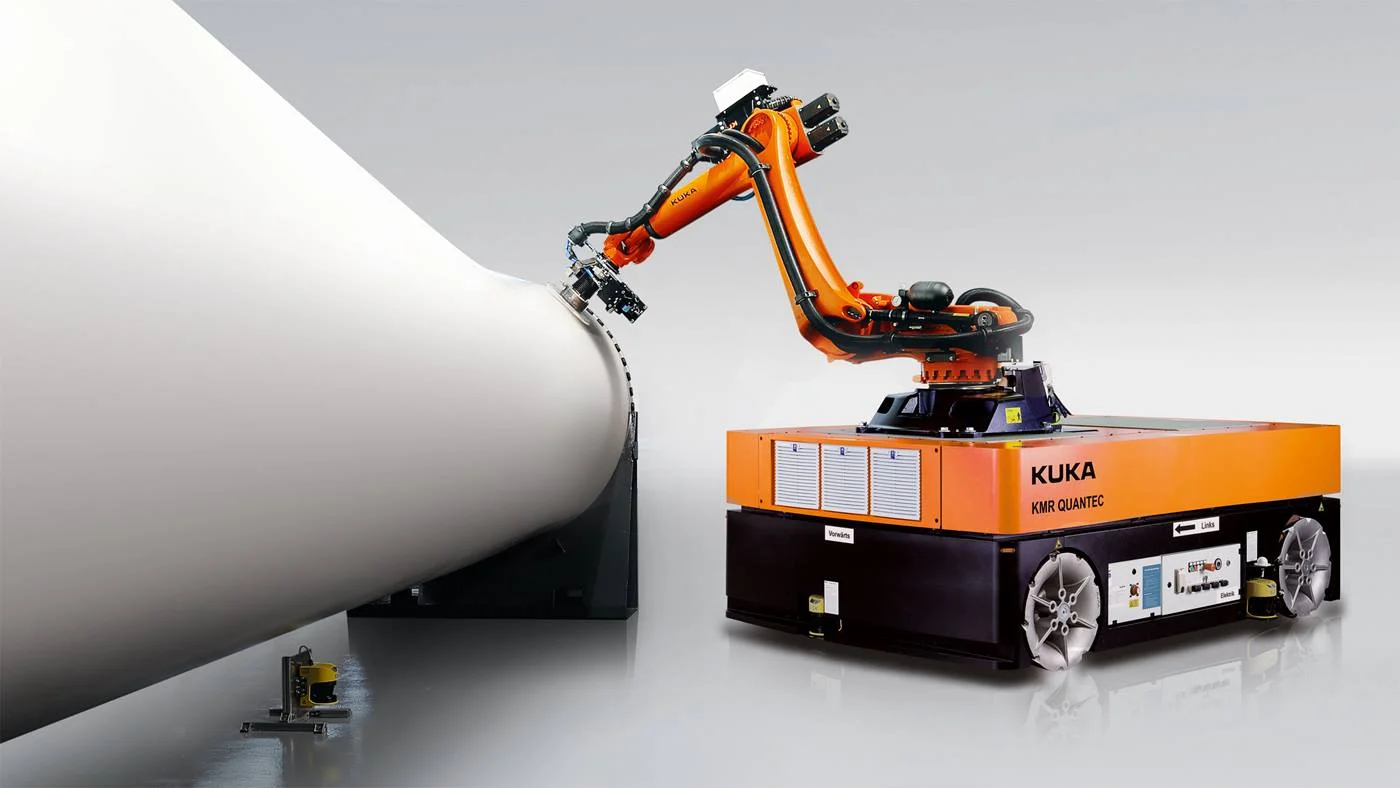
\includegraphics[width=0.4\linewidth]{Bilder/Grundlagen/industrie_mobiler_Roboter.png}}%
  \qquad
  \subfloat[][]{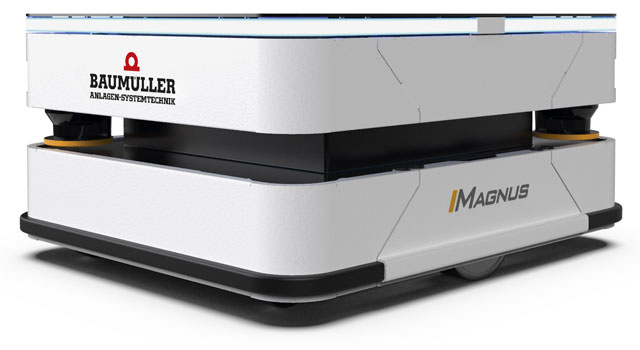
\includegraphics[width=0.4\linewidth]{Bilder/Grundlagen/bauMuellermagnus.jpg}}%
  \caption{Einsatz von mobilen Robotern in der Industrie (a) KMR QUANTEC \cite{KUKA_Roboter.2016} (b) Magnus der Firma Baumüller \cite{Baumueller.2021}}
  \label{fig:mobileRoboterIndustrie}
\end{figure}

\begin{figure}[]
  \centering
  \subfloat[][]{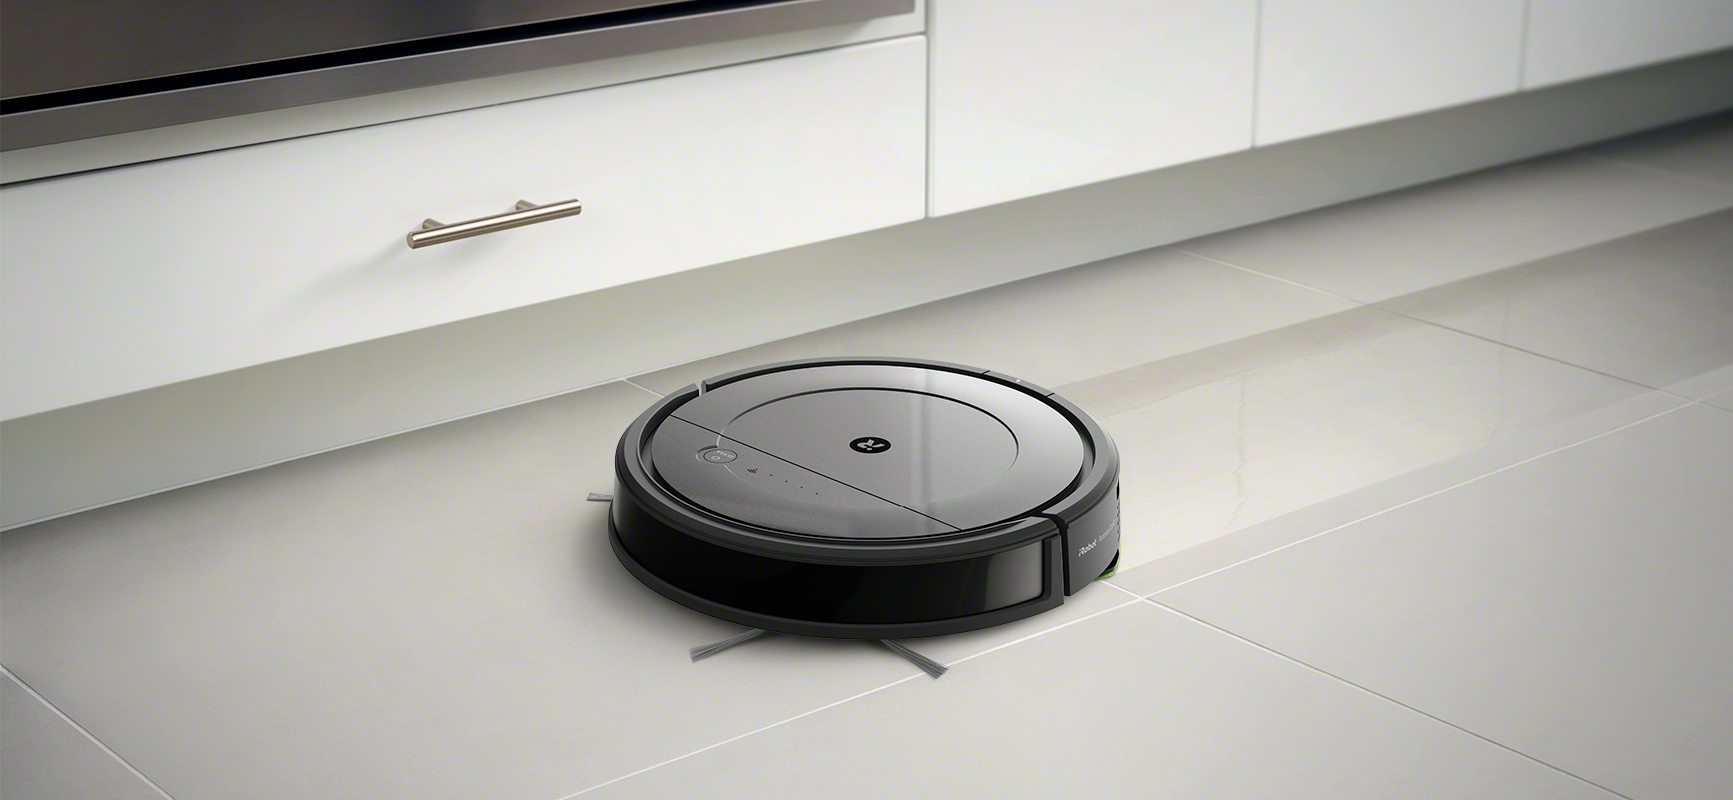
\includegraphics[width=0.4\linewidth]{Bilder/Grundlagen/IRobot_Wisch_Staubsauger.jpg}}%
  \qquad
  \subfloat[][]{\includegraphics[width=0.4\linewidth]{Bilder/Grundlagen/bosch_rasenmäroboter.jpg}}%
  \caption{Einsatz von mobilen Robotern in privaten Haushalten (a) Roomba Combo Saug- \& Wischroboter der Firma iRobot \cite{iRobot.2021} (b) Indego S+ 500 Roboter-Rasenmäher der Firma Bosch \cite{Boschdiy.2021}}
  \label{fig:mobileRoboterPrivaterHaushalte}
\end{figure}

Ein weiter Katastrophenfall ist die Corona Pandemie, die seit 2020 die ganze Welt in ihrem Bann hält. Die Pandemie hat viele Opfer gefordert, allein in Deutschland über 100.000, Stand 25.11.2021 \cite{tagesschau.25.11.2021}. Durch die leichte Übertragung hat sich das Virus zu einer Pandemie entwickelt. Die Corona Pandemie hat deutlich gemacht, das Keime und Viren auf Oberflächen an öffentlichen Orten und Arbeitsplätzen getötet werden müssen und dass es nicht nur ein Thema in Krankenhäusern ist. \cite{VDI_Corona_Roboter.2021} So konnte die autonome mobile Robotik sogar in der Pandemie an Wichtigkeit gewinnen. Es werden Serviceroboter entwickelt, die durch verschiedene Reinigungs- und Desinfektionsverfahren auf Oberflächen die Infektionsketten stoppen. Die Aufgabe der Desinfektionsroboter ist es zum Beispiel Türgriffe abzuwischen und im Anschluss über UV-Licht die Keime zu neutralisieren, sodass auch an schwer zugänglichen Stellen die Viren bzw. Keime getötet werden. Der mobile Roboter erkennt selbstständig durch Sensoren alle Objekte, die gereinigt werden müssen. \cite{VDI_Corona_Roboter.2021}
\newline
In dieser Arbeit soll eine Schnittstelle entwickelt werden, um die mobilen Roboter vereinfacht über Netzwerknachrichten zu bedienen. Dieses System soll als Grundlage dienen, um vereinfacht mobile Roboter in Bildungseinrichtungen als Lehrmaterial einzusetzen. Durch die standardisierten Schnittstellen können gezielt Benutzeroberflächen für unterschiedliche Anforderungen geschaffen werden, ohne die Implementierung am Roboter zu ändern.  


\section{Problemumfeld}
Die Abschlussarbeit entstand in Zusammenarbeit mit der Firma Kurt Hüttinger GmbH. Dabei war die Firma, während des Bearbeitungszeitraums, in einer wirtschaftlich schlechten Lage, da die Corona Pandemie das klein- und mittelständische Unternehmen belastete. Die Firma Hüttinger ist ein Unternehmen, das auf Messe- und Museumsbau spezialisiert ist. Da aber durch die Pandemie viele Ausstellungseinrichtungen geschlossen oder eingeschränkt sind, ist die Firma in eine wirtschaftliche Schieflage geraten, daher konnte der ursprüngliche mobile Roboter der Firma EduArt Robotik GmbH nicht bestellt werden. Die Arbeit wurde schließlich auf einen prototypischen Aufbau mithilfe vom Kobuki umgestellt. Infolgedessen wurde ein System angestrebt, das als Exponat in einem Museum bzw. einer Bildungseinrichtung ausgestellt werden kann. Die Abschlussarbeit soll eine offene Plattform bieten für die Bedienung von mobilen Robotern. Demnach können die Benutzeroberflächen für verschiedene Einrichtungen und Anforderungen entwickelt und geändert werden, ohne die roboternahe Implementierung zu ändern.  



\section{Zielsetzung} \label{sect:Zielsetzung}
In dieser Arbeit wird ein System ausgearbeitet, das in Bildungseinrichtungen zum Einsatz kommen könnte, um Kindern und Jugendlichen die Technik der allgegenwärtigen mobilen Roboter näher zu bringen. Dazu wird eine API entwickelt, die diese mobilen Roboter bedient und leichter zugänglich macht. So kann die Benutzeroberfläche zum Bedienen der mobilen Roboter offengehalten werden, da das API über Netzwerknachrichten bedient werden kann. Weiterhin werden in das API wichtige Funktionalitäten wie Hinderniserkennung implementiert. Dabei wird ein Kobuki Roboter für die experimentellen Tests verwendet.  